\begin{frame}{Podcast: Hours Rambled}
    \note{\scriptsize
    As we move forward, let's delve into the podcast episodes' duration.
    As mentioned before, the \emph{ÍSKISUR} were available on two platforms:
    \begin{itemize}
        \item the free streaming platform Alvarpið, a syndicated podcast on Nútíminn.is,
        \item and the subscription-based service, Storytel.
    \end{itemize}

    Both platforms launched with a teaser episode to set the stage for what the series would entail.
    As we proceeded, the approaches on the two platforms diverged a bit.
    \begin{itemize}
        \item On Alvarpið, the format was more freestyle, as I will discuss in a moment.
        \item However, when we transitioned to Storytel, we adopted a more systematic approach.
        The episodes followed a more rigorous structure, ensuring consistency in terms of time.
    \end{itemize}
    This structure is evident in the data.
    Over almost 4 years, we accumulated a hefty 7,762 minutes of engaging content,
        amounting to over 5 days of non-stop listening!
    On average, episodes on Storytel ran for just under an hour, about 10min longer than average on Alvarpið.

    Interestingly, none of the episodes on either platform ever crossed the 75-minute mark,
        showing our commitment to keep content concise and engaging.
    }
    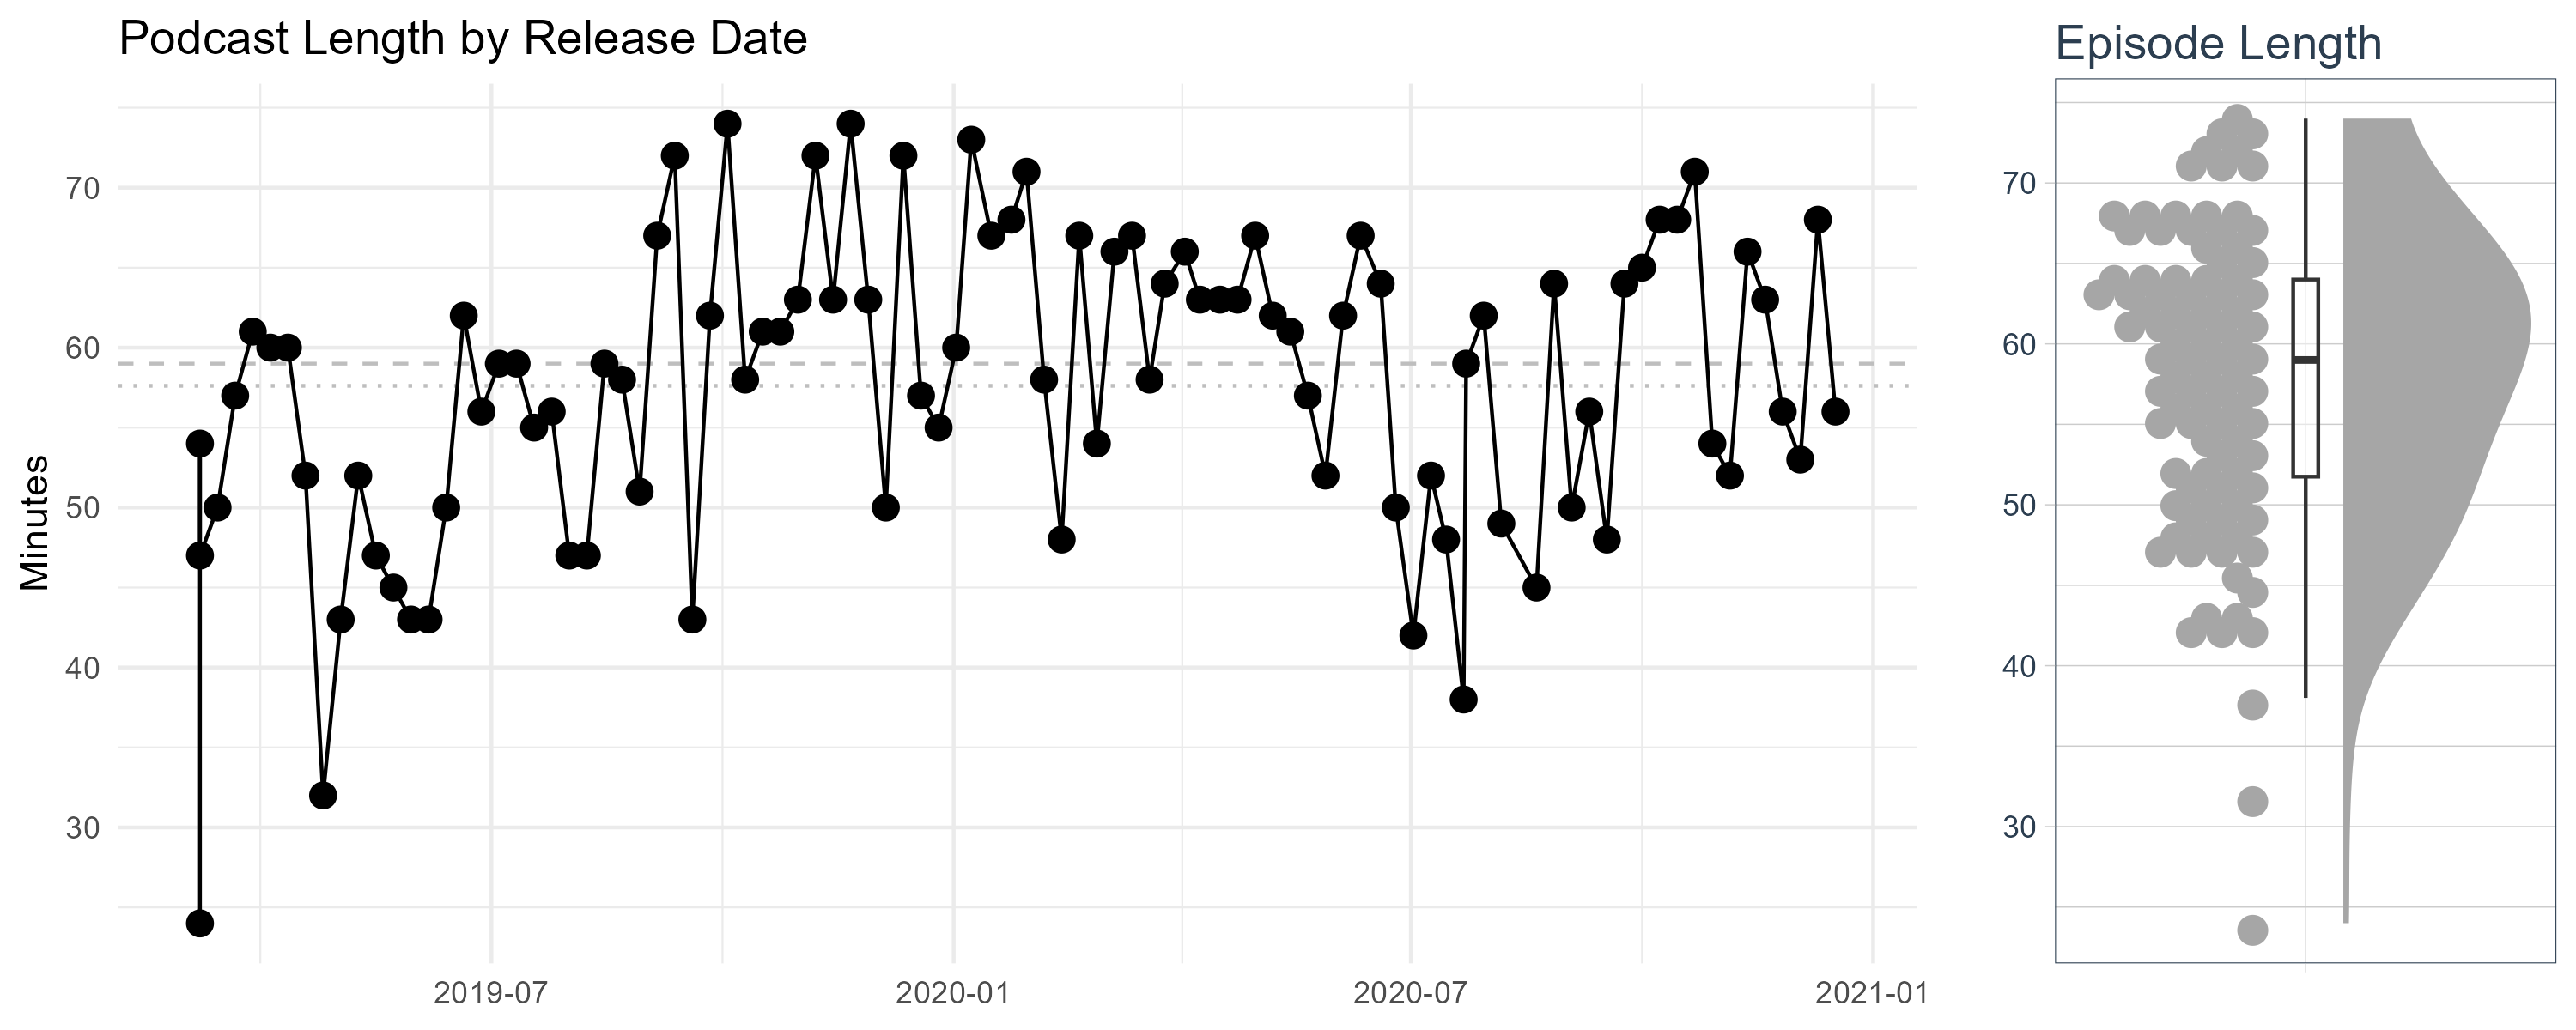
\includegraphics[width=\textwidth]{../rek-data-beers/R/figures/iskisur_length}
    \begin{itemize}
        \item Over a period of 45.8 months, there is 7,762 minutes of \emph{quality} content, or 5.4 days of continuous
        listening.
        \item Average length is 57.6 minutes on Storytel (48.5 on Alvarpið), but never surpassing 75 minutes.
    \end{itemize}
\end{frame}

\begin{frame}{Podcast on Alvarpið}
    \note{\tiny
    Let's get more granular and talk about our journey with the Alvarpið platform.
    As you can see on the chart, over 20 months we produced 46 episodes covering 5.5 books.

    Now, I wish I could provide you with precise listener figures for each episode.
    \begin{itemize}
    \item Most of our listeners were through podcast services like iTunes, when I requested data at the time
    the admin indicated a range of \emph{800-1000} listeners per episode.
    \item But what's still accessible to us is the listener count from \emph{Nútíminn} which was hosted
        through Mixcloud for those accessing via a browser. This data shows approximately 40 streams
        per episode.

    \item The Alvarpið phase was characterized by its free-form nature.
        We initially began with one chapter per episode but soon realized that this model wasn't
        sustainable. We then shifted to covering two chapters per episode, right up to the sixth book.
        Unfortunately, that book's coverage was curtailed prematurely due to a mix of challenges,
        including health issues within our team and logistical snags with file management.

    \item To give you a clearer picture, we were recording these episodes from two different locations:
        Kristín and I in Reykjavík, and Birna in Reyðarfjörður.
        The complexities of self-production were becoming evident.

    \item But as luck would have it, we were approached by Storytel at this juncture.
        They were venturing into podcasts and were keen to onboard us.
        This was a game-changer. Not just because they offered remuneration for our work
        (though, honestly, our passion for the project would have had us continuing for free!)
        but more so because they promised to handle the technicalities – synchronizing voice
        tracks and managing pitch adjustments.

    \item This meant we could redirect our energies to what we loved most: discussing the books and, of course,
        my personal favorite the cat segment towards the end.
    \end{itemize}
    }
    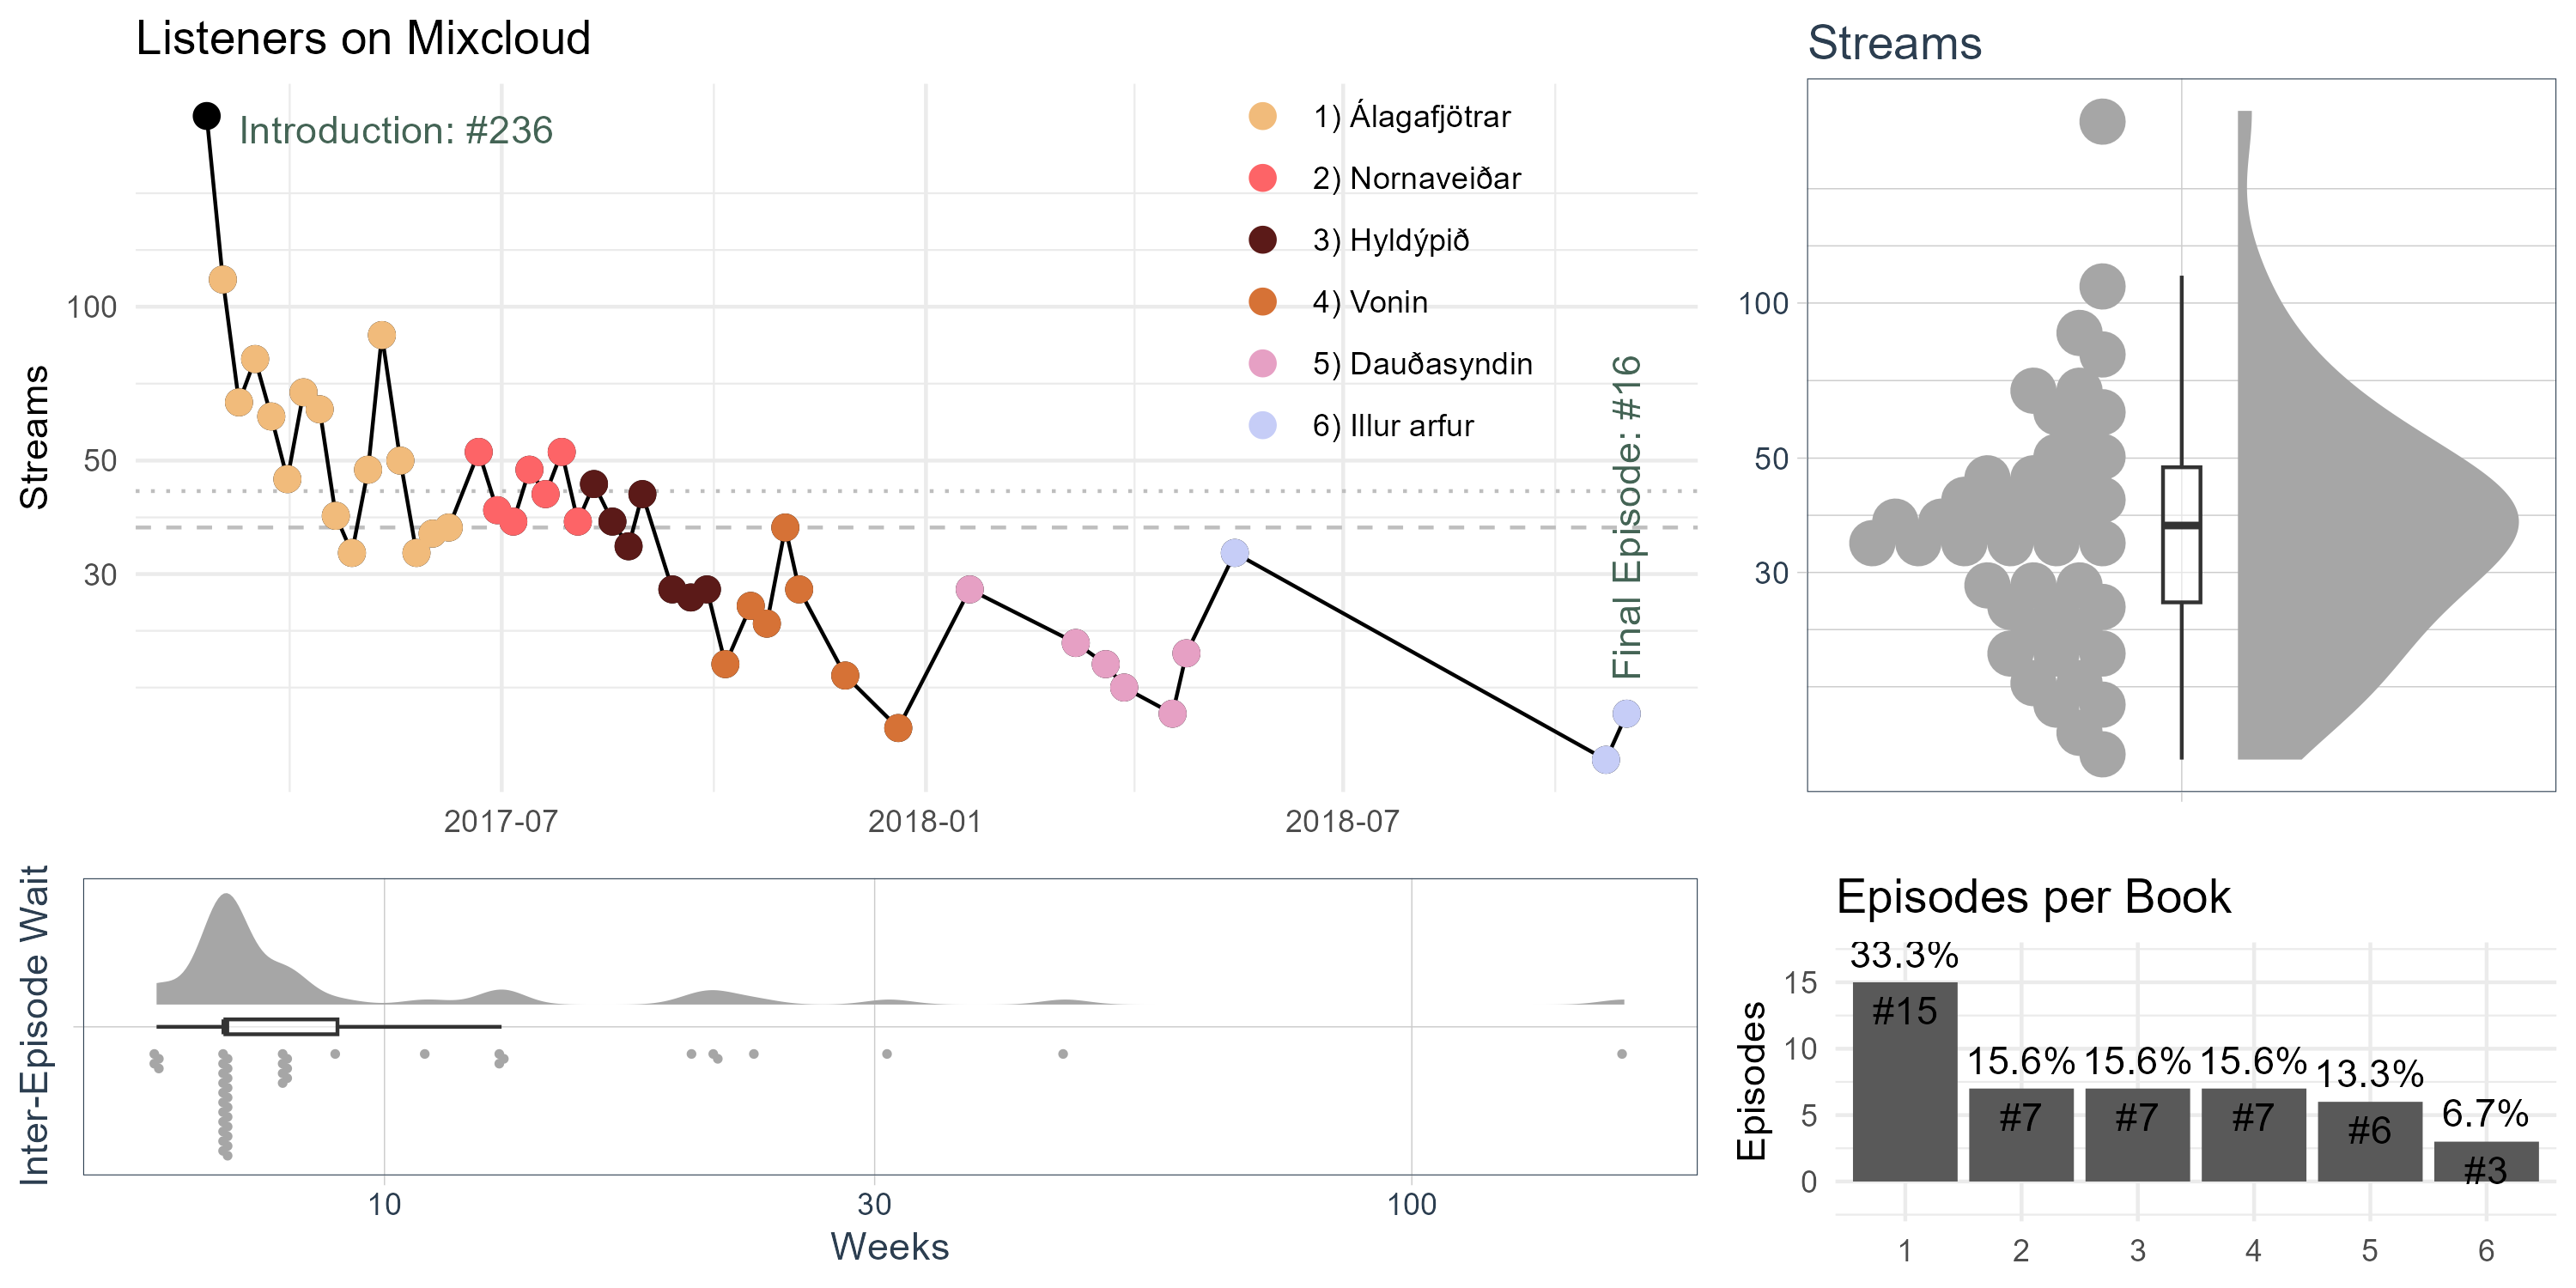
\includegraphics[width=\textwidth]{../rek-data-beers/R/figures/alvarpid_listeners}
    \vspace{-12pt}
    \begin{itemize}
        \item 46 episodes, 20 months, 5.5 books
        \item 2,231 minutes -- 37 hours -- 1.5 days of continuous listening
        \item Roughly 1,040 streams per episode (thereof ~40 via \url{nutiminn.is})
    \end{itemize}
\end{frame}

\begin{frame}{Podcast on Storytel: High Ratings}
    \note{\scriptsize
    Not only did Storytel lift the technical burdens off our shoulders,
        but our collaboration also bore fruit in terms of audience appreciation.
        The chart here displays our ratings on their platform. The numbers are truly heartening!
    \begin{itemize}
        \item On average, we have a stellar rating of 4.74 out of 5.
        \item The fact that 54 of our episodes have a perfect score of 5.0 speaks volumes.
        That's more than half of our episodes being rated as perfect by our listeners!
        \item It's also worth noting the outliers: only four episodes dipped below a 4.0 rating, with the lowest being 3.3.
        \item These numbers underscore the consistency of our content quality and, perhaps, the added value of having a professional platform backing us.
    \end{itemize}

    Given the challenges we faced with self-producing on Alvarpið, the seamless transition to Storytel and the ensuing high ratings gave us a rejuvenated sense of purpose.

    In retrospect, Storytel didn't just offer us a platform; they enhanced our user experience and,
        by extension, the experience of our audience.
    }
    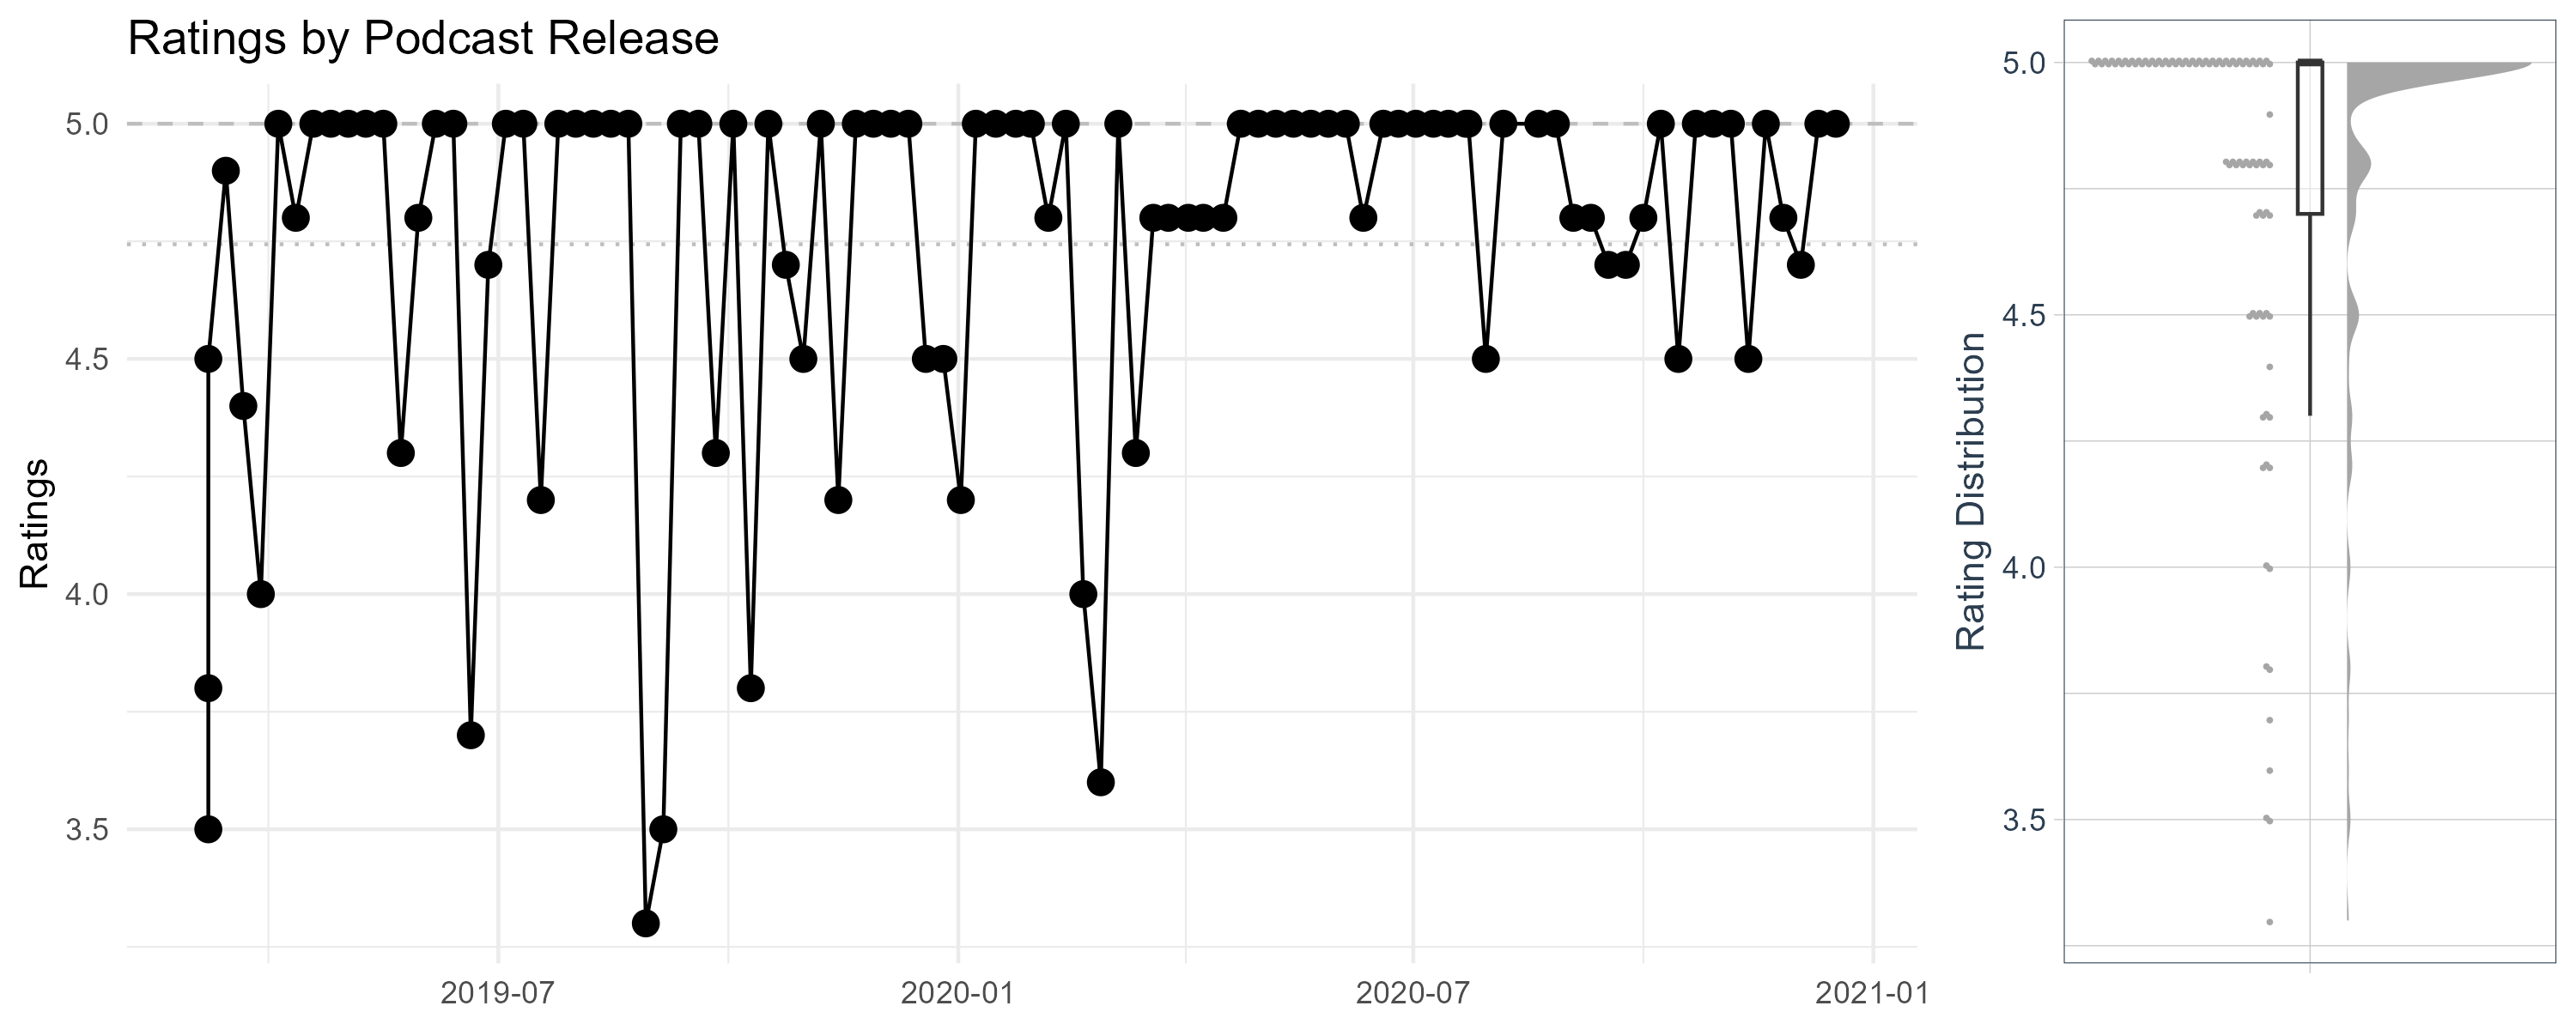
\includegraphics[width=\textwidth]{../rek-data-beers/R/figures/iskisur_ratings}
    \begin{itemize}
        \item Average rating: 4.74 out of 5
        \item 54 episodes with a perfect 5.0 score (56\% of total)
        \item Only 4 episodes with a rating below 4.0 (worst case 3.3)
    \end{itemize}
\end{frame}

\begin{frame}{Podcast on Storytel: Low Reviews}
    \note{\scriptsize
    Alright, let's ground ourselves with a touch of humility here. If you glance at the chart, you'll notice the not-so-overwhelming review count for our podcast. We might have had a high rating, but when it comes to reviews? We've got 444 in total, compared to the whopping 25,627 for the audiobooks. To put it in perspective, we were a tiny fish in a big Storytel pond.

    \emph{A confession}: I personally didn't always review our podcast. I admit, I tuned in for the first few episodes,
        bursting with pride that we were on the platform.
        But since I was already listening to all our episodes in post-processing
        (to jot down the hilarious text summaries, which you must read if you haven't already),
        I figured why double-dip? I suspect my co-hosts might've felt the same.

    Nevertheless, we celebrate our small victories.
    \begin{itemize}
        \item We've must have had at least \emph{one} active fan always reviewing our episodes,
        \item and there's a special place in our hearts for the \emph{four} fans who consistently
        dropped in with their feedback.
    \end{itemize}

    In essence, our podcast was an intimate book club, where we referred to our listener as our \emph{only} fan.
        So, even if we sometimes talked over you (or our co-hosts, whoops!), after all it's a podcast,
    know that we always appreciated your company.

    So, cheers to our only fan, wherever you are!
    }
    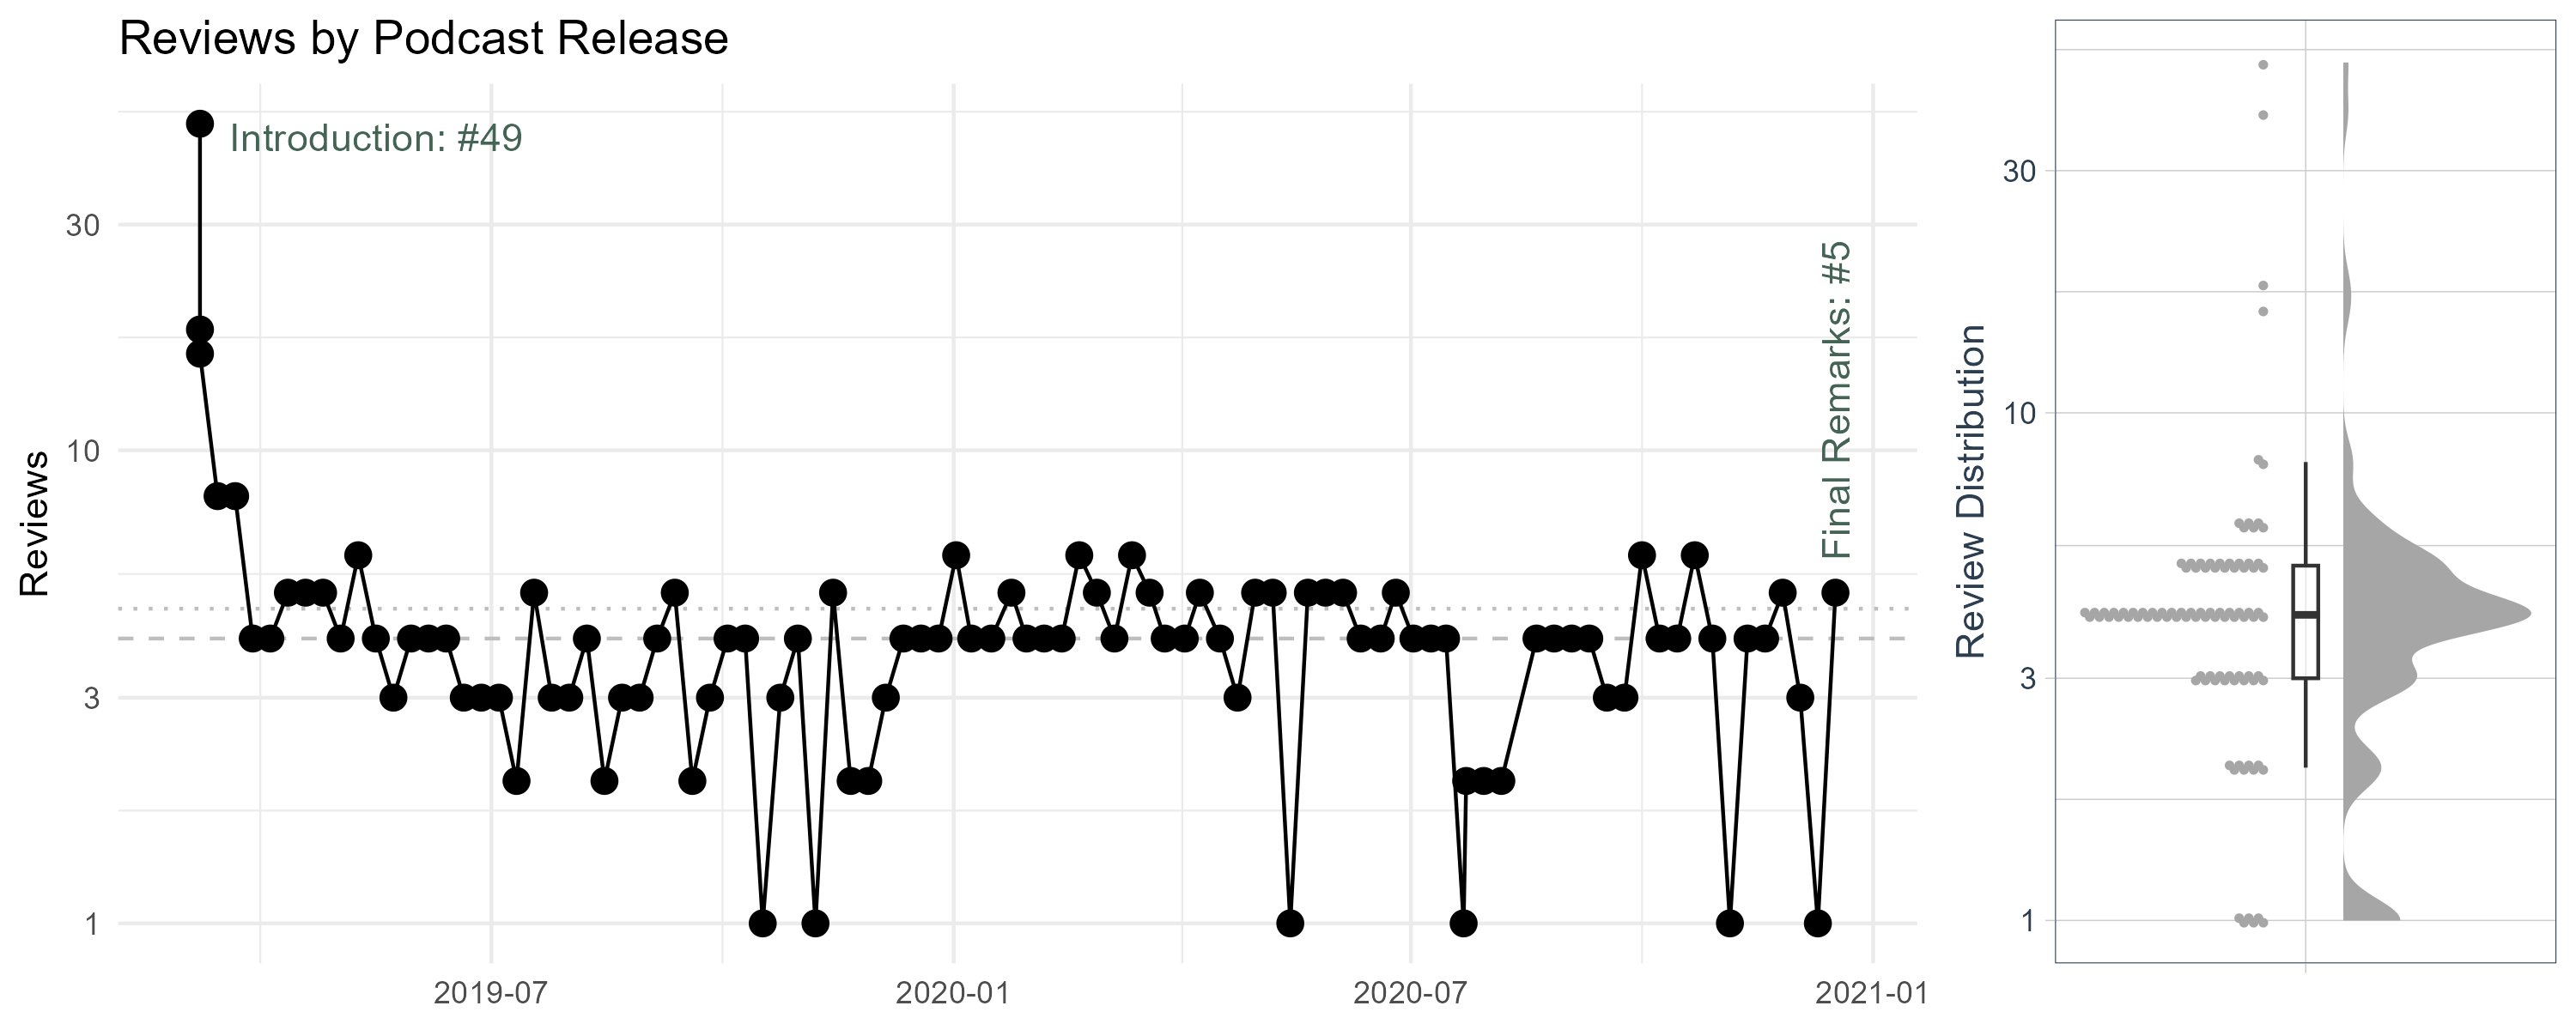
\includegraphics[width=\textwidth]{../rek-data-beers/R/figures/iskisur_reviews}
    \begin{itemize}
        \item Number of reviews: 444 total (25,627 for the audiobooks)
        \item At least one active fan throughout the period
        \item Four regular fans who consistently provided review
    \end{itemize}
\end{frame}

\begin{frame}{Podcast Platform Comparison}
    \note{
    As we conclude, here's a bird's-eye view of our podcast journey:
    \begin{itemize}
        \item We went from crafting 46 episodes on Alvarpið to a staggering 96 on Storytel.

        \item The average episode length slightly increased on Storytel, hinting at our growing comfort and expanded discussions.

        \item Notice the stark difference in release consistency: Alvarpið saw gaps as long as 161 days, while Storytel never went beyond a 14-day hiatus.

        \item In terms of overall engagement, both platforms gave us roughly 20 months of active podcasting each, but let's not forget that 4.1-month pause we took in between.
    \end{itemize}

    Most importantly, we had a blast throughout the journey, and we managed to cover all 47 books in the series in record time (in true Margit fashion)
    }
    \begin{table}[]
        \begin{tabular}{l|rr|rr|rrr|r}
            & \rotatebox{90}{Episodes} & \rotatebox{90}{Books} &
            \rotatebox{90}{Total Running Time (hours)} & \rotatebox{90}{Average Length (min)} &
            \rotatebox{90}{Median Days to Next}
            & \rotatebox{90}{Average Days to Next}  & \rotatebox{90}{Max Days to Next}  &
            \rotatebox{90}{Months Active} \\
            \midrule
            Alvarpið & 46  & 6  & 37.2  & 48.50 & 7 & 13.69 & 161 & 20.3  \\
            Storytel & 96  & 47 & 92.2  & 57.61 & 7 & 6.85  & 14  & 21.4  \\
            \midrule
            & 142 &    & 129.4 &       &   &       &     & 45.8*
        \end{tabular}
    \end{table}

    \vfill
    \footnotesize{*4.1 months hiatus between Alvarpið and Storytel}
\end{frame}
